%%%%%%%%%%%%%%%%%%%%%%%%%%%%%%%%%%%%%%%%%%%%%%%%%%%%%%%%%%%%%%%%%%%%%%%%%%%%%%%%%%%%%%%%%%%%%
%%									ANNEXES 												%
%%%%%%%%%%%%%%%%%%%%%%%%%%%%%%%%%%%%%%%%%%%%%%%%%%%%%%%%%%%%%%%%%%%%%%%%%%%%%%%%%%%%%%%%%%%%%
\chapter{Annexes}
\minitoc

%%%%%%%%%%%%%%%%%%%%%%%%%%%%%%%%%%%%%%%%%%%%%%%%%%%%%%%%%%%%%%%%%%%%%%%%%%%%%%%%%%%%%%%%%%%%%
\section{Dérivation des équations pressions/flux du modèle}
\label{sec:deriveq}
Lors de la définition de l’équation de conservation de la quantité de mouvement, nous avons
évoqué la situation dans les connexions en Y (un tube se subdivise en deux). Nous décrirons ici le détail
du calcul permettant d’aboutir à l’équation correspondante dans cette situation.
%%%
\begin{figure}[!t]
\centering
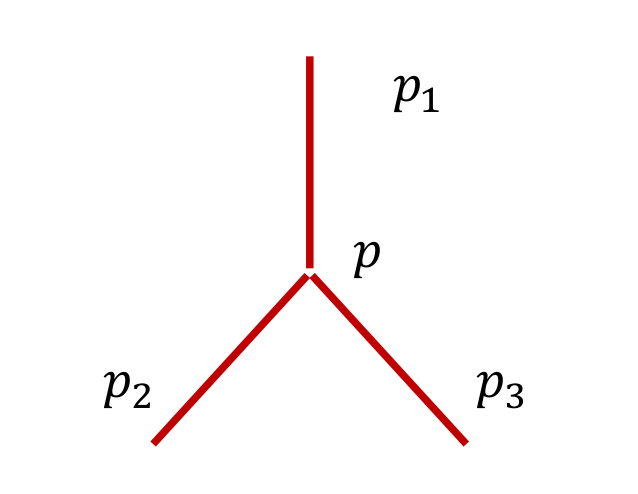
\includegraphics[width=10cm]{A_1_schema_Y}
\caption{Notation employée dans la structure en Y. p représente la pression à l’intersection des trois tubes, et p1 , p2 , et p3
les pressions dans les tubes.}
\label{fig:A_1_schema_y}	
\end{figure}
Soit la pression $p$ commune à l’intersection et les pressions $p_1$ , $p_2$ , et $p_3$ de chaque tube (Figure~\ref{fig:A_1_schema_y}). On
a, dans une approximation linéaire :
\begin{eqnarray}
p_1\,-\,p\,-\,\frac{a_1}{2}f_{out}=0\\
p_2\,-\,p\,-\,\frac{a_2}{2}f_{out}=0\\
p_3\,-\,p\,-\,\frac{a_3}{2}f_{out}=0\\
\end{eqnarray}
Avec $a$ la résistance (dont on ne prend ici que la moitié puisque les $p_i$ sont mesurés au milieu du tube)
et $f$ les flux (voir Figure~\ref{fig:4_8_param_tubes}). Le bilan des flux à l’intersection est nul : $f_{out1} + f_{out2} + f_{out3}=0$. Nous
avons donc 4 équations pour 4 inconnues (les flux). Ainsi on résout et on trouve :
\begin{eqnarray}
\frac{a_2}{2}(p_1-p_3)\,+\,\frac{a_3}{2}(p_1-p_2)\,-\,\beta_{123}f_{out1}\,=\,0;
\frac{a_3}{2}(p_2-p_1)\,+\,\frac{a_1}{2}(p_2-p_3)\,-\,\beta_{123}f_{out2}\,=\,0;
\frac{a_1}{2}(p_3-p_2)\,+\,\frac{a_2}{2}(p_3-p_1)\,-\,\beta_{123}f_{out3}\,=\,0;
\end{eqnarray}
avec $\beta_{123}=\frac{a_1}{2}\frac{a_2}{2}+\frac{a_1}{2}\frac{a_3}{2}+\frac{a_2}{2}\frac{a_3}{2}$, qui vérifie bien $f_{out1} + f_{out2} + f_{out3}=0$. Nous retrouvons ainsi l’Équation~\ref{eq:ley} décrite précédemment.
%%%
%%%
%%%
\section{Filtrages et traitements d’images}
Les acquisitions réalisées au sein de notre protocole tel que défini précédemment aboutissent
à des images de résolutions et parfois d’orientations différentes. Il nous sera donc indispensable de
trouver les transformations permettant de superposer une image à une autre, c’est-à-dire de les
ramener dans un espace commun. Les procédures classiques en traitement d’image IRM qui
permettent ces transformations sont le réalignement, la coregistration et la normalisation.\\
Dans le cadre de la thèse, l’ensemble des traitements d’image ont été réalisés en utilisant
MATLAB (MathWorks, Natick, MA) et SPM8 (Statistical Parametric Mapping; the Wellcome Trust
Center for Neuroimaging, UK). En effet, SPM8 constitue la bibliothèque de programmation sous
MATLAB de référence en la matière et propose un grand nombre de fonctions assurant le traitement
des données IRM. Quelques-unes de ces fonctions seront souvent utilisées, il convient donc de les
décrire.
%%
%%%
\subsection{Réalignement}
Le réalignement comme son nom l’indique, permet de réaligner deux volumes d’un même
sujet dont le contraste est identique. Un sujet bouge toujours (même très faiblement) dans l’IRM. Dans
les acquisitions répétées telles que l’ASL, durant lesquelles des couples d’images contrôles et
marquées sont récupérés au cours du temps, tout mouvement engendrera des erreurs pouvant
impacter le résultat lors du calcul de la différence. Il est donc indispensable de s’assurer que le sujet
n’a pas bougé, ou le cas échéant, de corriger ce mouvement.\\
%%%
\begin{figure}[!t]
\centering
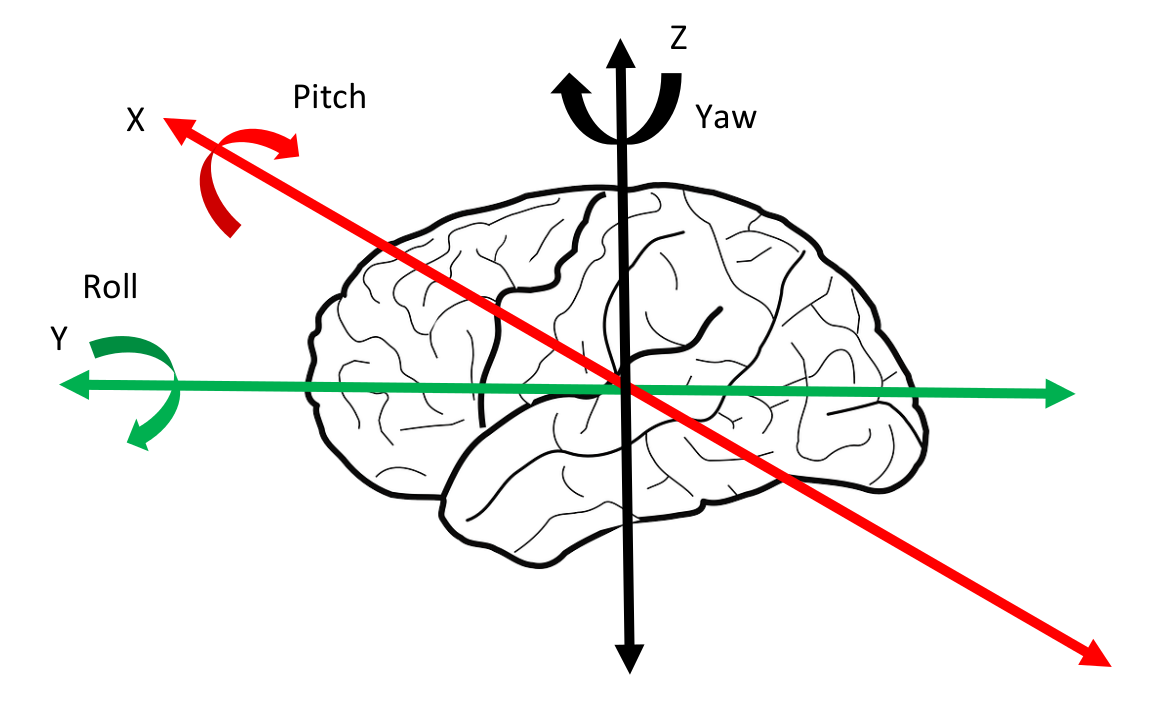
\includegraphics[width=10cm]{A_2_realignement}
\caption{Illustration des transformations possibles dans un réalignement.3 translations, 3 rotations.}
\label{fig:A_2_realignement}	
\end{figure}
Pour réaliser un réalignement, on commence par sélectionner une image dite de référence
correspondant à un volume représentatif de l’acquisition. Tous les autres volumes seront alors
transformés pour correspondre à celui-ci. Le processus s’effectue en deux étapes. La première est
purement géométrique : on suppose que toutes les images montrent le même cerveau, donc une
simple transformation rigide est suffisante. Nous recherchons ainsi les translations (selon X, Y et Z) –
rotations (selon X, Y et Z) nous permettant de rendre superposable nos volumes (Figure~\ref{fig:A_2_realignement}) : c’est
l’alignement (« registration »), qui va déterminer les 6 paramètres qui décrivent la transformation
rigide entre l’image source et la référence. La seconde étape est constituée d’un ré-échantillonnage
de l’image visant à aligner le maillage des voxels avec celui de l’image de référence, les rendant
superposables : c’est l’étape dite de redécoupage ou « reslicing ».\\
L’algorithme est itératif, constitué d’une succession de petits déplacements de l’image. A
chaque étape, une mesure de l’écart entre l’image à réaligner et la référence est calculée. On utilise
en général la somme des différences au carré des voxels (\cite{Ashburner1997}). Trouver le meilleur alignement consiste
à identifier les paramètres qui minimisent cette somme. Il s’agit d’un problème classique
d’optimisation. La convergence vers la solution est assurée par une méthode de Gauss-newton. Dans
cette approche, le minimum est estimé en réalisant un ajustement quadratique à chaque itération
(Figure~\ref{fig:A_3_gaussnewton}). La correction du mouvement est effectuée à chaque étape à une résolution plus fine que
celle des deux images. \\
%%%
\begin{figure}[!t]
\centering
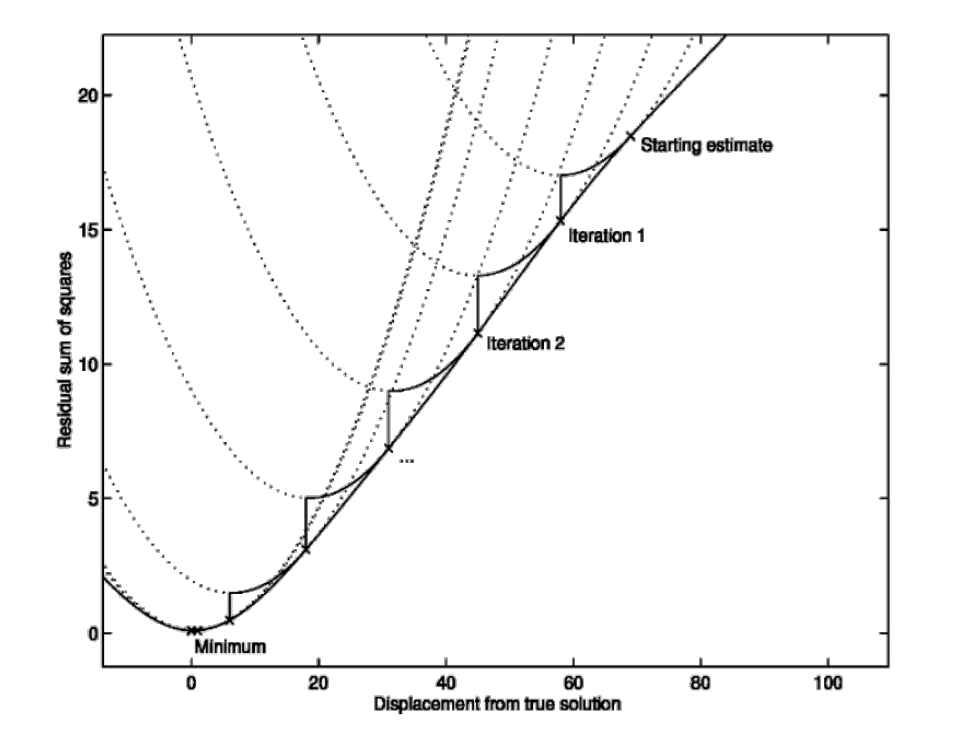
\includegraphics[width=10cm]{A_3_gaussnewton}
\caption{Illustration de l’optimisation de Gauss-newton dans le réalignement.}
\label{fig:A_3_gaussnewton}	
\end{figure}
La seconde étape consiste à appliquer à l’image à réaligner la transformation estimée. La
précision du réalignement étant inférieure à celle du voxel, il est donc nécessaire de ré-échantillonner
l’image à des positions intermédiaires entre les centres des voxels. Cela requiert une interpolation
pour estimer l’intensité d’un nouveau voxel sur la base des anciens. Différentes méthodes
d’interpolations sont disponibles, toutes des variantes d’une simple interpolation linéaire. On
distinguera entre autre l’interpolation par les plus proches voisins, qui est la méthode la plus rapide,
et qui assure une conservation de la valeur des voxels ; et l’interpolation trilinéaire, la plus utilisée en
IRM et l’une des plus efficace mais qui est plus longue à calculer.\\
Notons que dans la problématique spécifique du réalignement ASL, une nouvelle difficulté
apparait liée aux différences de signal inhérentes à la méthode entre les images contrôles et les images
marquées. Dans ce cas, le réalignement peut générer des déplacements artéfactuels dis « zig-zag »
entre les deux images. Il devient donc important de réaligner indépendamment les images contrôles
et les images marquées puis de refaire le lien entre les deux groupes à postériori (\cite{Wang2008}). Des
optimisations du réalignement de SPM ont été réalisées pour l’ASL (\cite{Wang2012}).\\
%%%
%%%
\subsection{Co-registration}
En imagerie IRM, on appelle spécifiquement réalignement, le traitement précédemment
exposé qui permet de superposer deux images disposant du même contraste. Lorsque les deux images
ont intrinsèquement un contraste différent (T$_1$ versus T$_2$ par exemple), on parle de co-registration.
Lors d’acquisitions contenant de multiples modalités comme la nôtre, il est important de les
positionner dans le même espace de façon à être en mesure de naviguer facilement d’une image à
l’autre, et de les superposer. Cependant, du fait des différences d’intensités pour une même région, la
minimisation des scores de différences entre les images, tel qu’elle est faite dans un simple
réalignement, ne permet pas d’aboutir à un résultat satisfaisant. Il faut donc trouver une
transformation de corps rigide (6 paramètres) qui relie les deux images sans passer par la minimisation
simple de la différence des intensités.\\
Comme pour le réalignement, le processus de co-registration est ramené au problème de
l’optimisation d’une fonction de coût. Une première approche pour calculer cette fonction de coût
consiste à extraire indépendamment des deux images une même information générique, par exemple
la segmentation des différents tissus. On minimise ensuite la moyenne des différences au carré de ces
informations génériques (\cite{Ashburner1997}. Une autre approche consiste à calculer l’information mutuelle. Il s’agit
d’un concept issu de la théorie de l’information. Pour deux images données, l’information mutuelle
permet de quantifier leur ressemblance. Son calcul est basé sur la densité conjointe de probabilité des
niveaux de gris des deux images. Pour cela on calcule un histogramme conjoint des niveaux de gris. Les axes de l’histogramme représentent l’intensité des voxels sur chaque image ; chaque point (a,b) du
plan correspond à une intensité a sur la première image et à une intensité b sur la deuxième. 
%%%
\begin{figure}[!t]
\centering
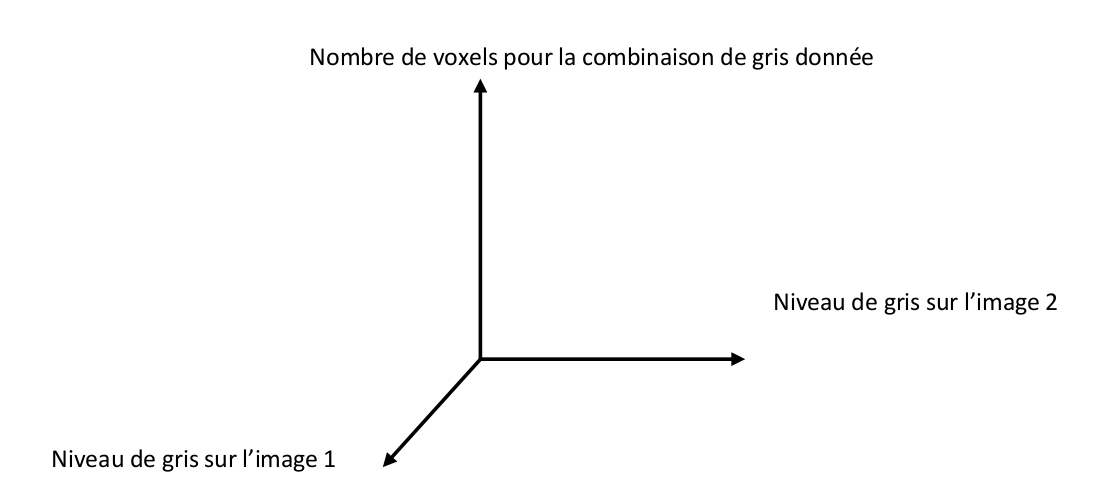
\includegraphics[width=5cm]{A_4_hist_conj}
\caption{Axes d'un histogramme conjoint. Le nombre de voxel pour une combinaison de niveau de gris donnée peut être
représenté par une couleur.}
\label{fig:A_4_hist_conj}	
\end{figure}
On
attribue à chaque point un niveau de gris, en fonction du nombre total de voxels ayant une intensité a
sur la première image et une intensité b sur la deuxième (Figure~\ref{fig:A_4_hist_conj}). Lorsque les images sont alignées,
certains points de l’histogramme ont un niveau de gris élevé et les autres proche de 0, puisque tous
les voxels coïncident (Figure~\ref{fig:A_5_ex_hist}). En revanche, lorsque les images ne sont pas bien alignées, le nombre
de coïncidences diminue et le niveau de gris se disperse sur l’histogramme.\\
%%%
\begin{figure}[!t]
\centering
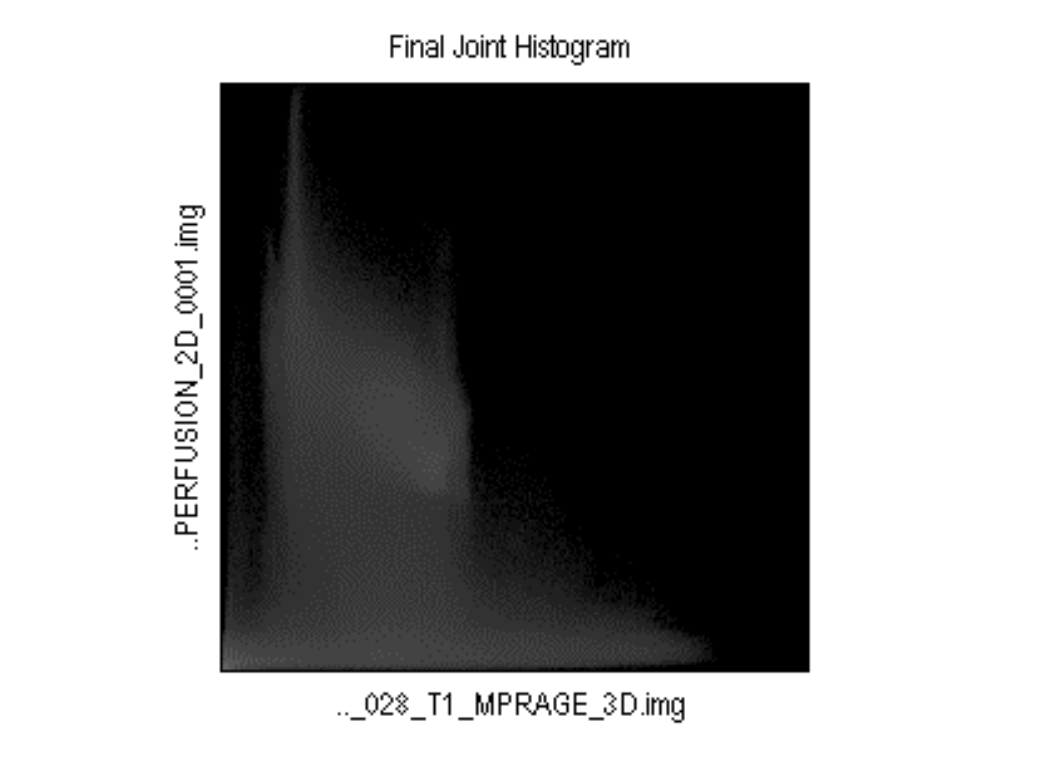
\includegraphics[width=5cm]{A_5_ex_hist}
\caption{Exemple d'histogramme conjoint obtenu par SPM après coregistration d'une image EPI d'ASL et d'un T$_1$.}
\label{fig:A_5_ex_hist}	
\end{figure}
L’information mutuelle permet de quantifier cette information (\cite{Collignon1995}). Elle se calcule directement à
partir de l’histogramme conjoint comme suit :
\begin{equation}
MI\,=\,\sum_{i,j}p_{ij}log\biggl(\frac{p_{ij}}{p_ip_j}\biggr)
\end{equation}
avec $i$ et $j$ les coordonnées sur l'histogramme conjoint, $p_{ij}$ la probabilité qu’un point pris au hasard dans
l’image soit la combinaison du niveau de gris $i$ sur l’image 1 et $j$ sur l’image 2, $p_i$ la probabilité pour un
$i$ donné que l’on trouve un point de niveau de gris $i$ sur l’image 1, $p_j$ la probabilité pour un $j$ donné que
l’on trouve un point de niveau de gris $j$ sur l’image 2. C’est cette information mutuelle que l’on
cherchera à maximiser.\\
%%%
%%%
\subsection{Normalisation}
Comme les traitements précédents, la normalisation cherche à trouver la transformation
permettant de superposer deux images. La normalisation est utilisée dans des contextes de
comparaisons de groupes, lorsqu’il convient de rapporter les images de différents sujets dans un
espace commun afin de soit les superposer à un atlas défini dans cet espace, soit réaliser des analyses
dites de Voxel Based Morphometry (VBM) où l’on compare un à un les voxels (\cite{Mechelli2005}) qui doivent donc
correspondre à la même coordonnée. De même cela permet de rapporter des résultats dans un
système de coordonnées standardisé (Talairach etc.). L’espace Talairach par exemple, est défini par un
certain nombre de marqueurs tel que les commissures antérieure et postérieure qui déterminent
l’angle de la boite autour de l’axe $X$, le plan sagittal défini la séparation gauche droite (\cite{Talairach1988}). Dans le cadre de notre étude, en dépit du fait qu’il n’y a pas à priori de comparaisons de groupe, cette étape
est rendue indispensable du fait de son intégration nécessaire dans le processus de segmentation des
tissus (voir après). Ce processus repose en effet sur la comparaison avec des cartes de densité de
probabilité dans un espace normalisé.\\
Pour effectuer ce traitement, il n’est plus possible d’utiliser les simples approches
d’alignement de corps rigides puisque l’image à normaliser n’a aucune raison d’être de la même forme
que l’image de référence (ici appelée template). En plus des transformations de rotations et
translations, on doit intégrer la mise à l’échelle selon les trois axes séparément, ainsi que des
déformations cisaillements. On aboutit à une transformation affine 3D à 12 paramètres. De plus, une
seconde étape de transformation non linéaire permet de gérer les différences d’échelle plus faible
dans l’anatomie du cerveau. Le modèle de cette seconde étape utilise des déformations qui consistent
en une combinaison linéaire de fonctions de bases périodique basse fréquence.\\
%%%
\begin{figure}[!t]
\centering
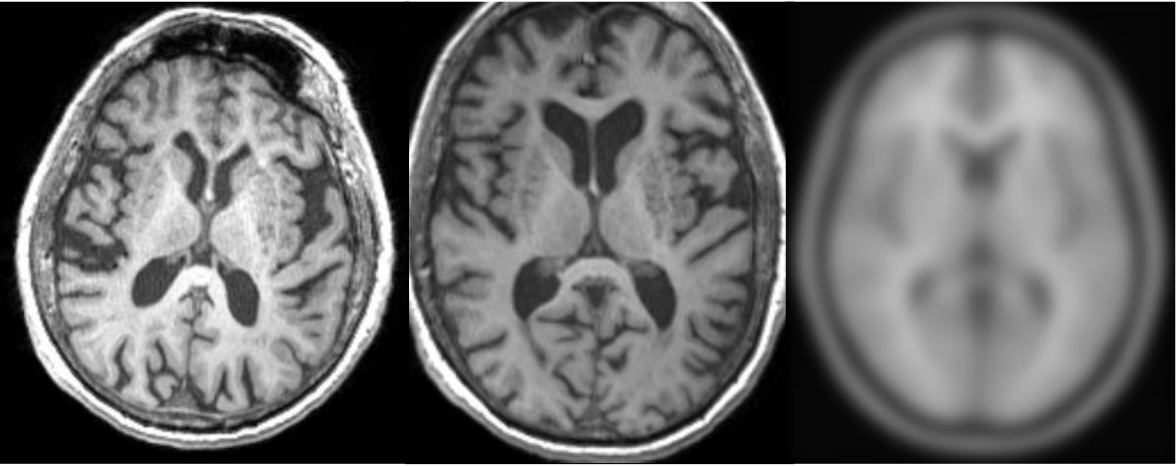
\includegraphics[width=10cm]{A_6_normalisation}
\caption{Résultat de la normalisation d'une imagerie T$_1$. De gauche à droite, l'image brute, l'image normalisée, et le
template T$_1$ (SPM) utilisé.}
\label{fig:A_6_normalisation}	
\end{figure}
SPM utilise une approche basée sur l’intensité des voxels pour réaliser la normalisation (\cite{Ashburner2003})
contrairement à d’autres outils tels que FreeSurfer qui utilisent une approche basée sur l’anatomie
(\cite{Buckner2004}). SPM propose un template T$_1$ de référence permettant de normaliser ce type d’imagerie dans
l’espace MNI (Montreal Neurological Institute) (Figure~\ref{fig:A_6_normalisation}). Cet espace a été pour la première fois
défini à partir de 241 IRM de sujets sains. Sur ces images différents marqueurs ont été identifiés puis
les images ont été mises à l’échelle et réchantillonnées afin de faire correspondre ces marqueurs à
ceux de l’atlas de Talairach (\cite{Collins1995}).\\
SPM propose maintenant une nouvelle approche appelé DARTEL, pour Diffeomorphic
Anatomical Registration Through Exponentiated Lie Algebra. Cette nouvelle méthode permet entre
autres la création d’un template adapté à une cohorte donnée, et la normalisation des images sur ce
template. Les informations de déformations sont stockées dans un seul fichier « flow field » (champ de vecteurs) considéré constant dans le temps (\cite{Ashburner2007}). Cela permet une normalisation annoncée comme
plus fine, cependant les données se retrouvent dans un espace qui est propre à leur cohorte (du fait
de la création du template), qui est légèrement différent de l’espace couramment utilisé : l’espace
MNI. Une étape additionnelle de recalage vers cet espace est donc requise. Cet outils se positionne de
plus en plus comme la référence en terme de normalisation (\cite{Klein2009}).
%%%
%%%
\subsection{Segmentation}
Au niveau cérébral, on distingue principalement trois tissus : la matière grise, la matière
blanche et le liquide cérébro-spinal. La segmentation vise le plus souvent à identifier ces tissus dans
l’image IRM. En effet, en pondération T$_1$, ces tissus disposent d’un contraste différent. Une fois ces
tissus identifiés il sera possible de réaliser l’extraction du cerveau pour éliminer le crâne.\\
Deux grandes approches de segmentation existent (Figure~\ref{fig:A_7_segmentations}). Les approches orientées
contours, qui comme leur nom l’indique se focalisent sur la recherche des limites des régions sur la
base de modèles déformables (snakes, level-sets) ou de morphologie mathématique (gradient morphologique, ligne de partage des eaux) (\cite{Scherrer2008}). Et les approches orientées régions, plutôt basées
sur la définition de régions selon les niveaux d’intensités de l’image (croissance de régions, K-mean
etc.). La recherche de contours est particulièrement adaptée à la détection du crâne et de la périphérie
du cerveau. Des modèles déformables sont d’ailleurs utilisés au sein de l’outils BET (Brain Extraction
Tool) de FSL permettant l’extraction du cerveau (\cite{Smith2002}). Pour segmenter les différents tissus, l’approche
orientée région est privilégiée. SPM se base sur une approche de segmentation unifiée probabiliste
(\cite{Ashburner2005}) basée sur l’intensité des voxels et l’utilisation de cartes de probabilités des tissus (TPM) obtenues
à partir de nombreux sujets sains. C’est une méthode intimement liée au DARTEL. Elle fait partie des
approches les plus robustes à l’heure actuelle (\cite{Malone2015}). 
%%%
\begin{figure}[!t]
\centering
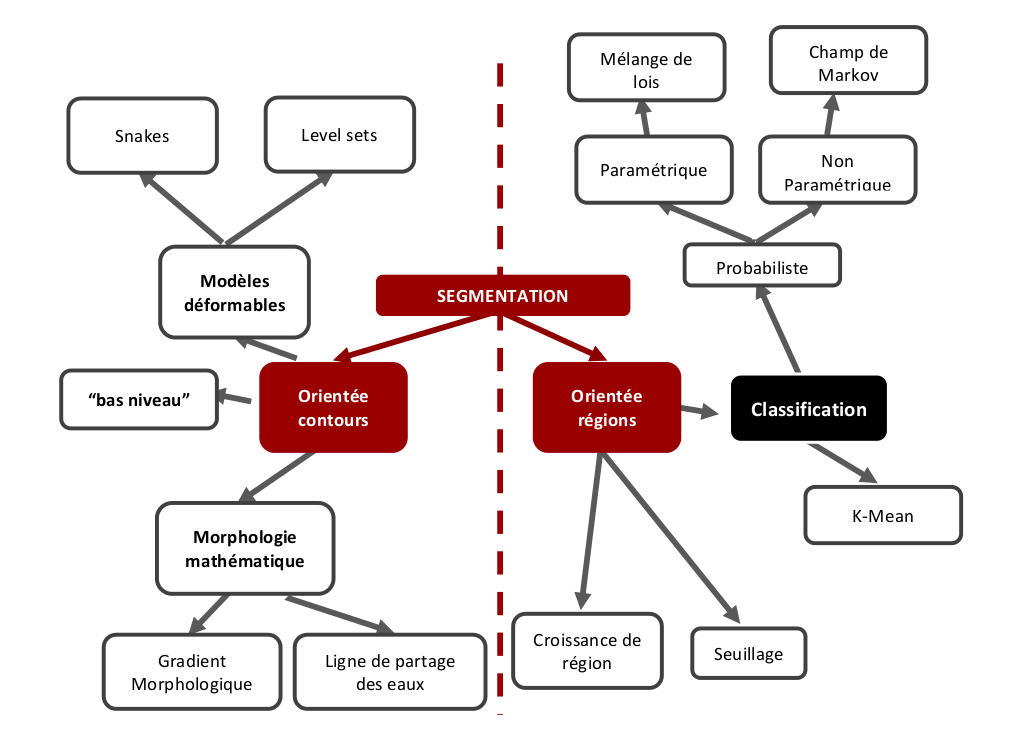
\includegraphics[width=10cm]{A_7_segmentations}
\caption{Présentation des différents algorithmes de segmentation disponibles. Adapté de \cite{Scherrer2008}}
\label{fig:A_7_segmentations}	
\end{figure}
Dans une première étape, on cherche à décrire
l’histogramme des voxels comme une superposition de distributions gaussiennes. En effet si l’on
regarde l’histogramme d’une image pondéré en T$_1$, on observe la présence de plusieurs pics
correspondant aux tissus de contraste différents. Une fois les gaussiennes obtenues, elles sont
normalisées par l’histogramme total afin d’obtenir les probabilités d’appartenance. On obtient ainsi
une segmentation « brute ». Cette étape est cependant très sensible aux inhomogénéités de signal
dans l’image, qui résultent de la non uniformité de $B_0$, de la bobine RF, d’artéfacts etc. (\cite{Kwan1999}). SPM
intègre donc une étape préalable d’estimation et de correction de ces biais permettant de limiter leur
impact.\\
Une fois cette première segmentation obtenue, elle est comparée aux cartes de probabilités
apriori disponibles (TPM) en utilisant une approche bayésienne. L’image en niveau de gris et la
segmentation (« étiquettes ») seront considérée comme les réalisations de deux champs aléatoires $Y
= \{y_1, ... y_i, ... y_N\}$ et $Z = \{z_1, ... z_i, ... z_N\}$. On a alors :
\begin{equation}
p(Z\mid Y,\phi)\,=\,\frac{p(Y\mid Z,\phi_Y) p(Z\mid \phi_Z)}{p(y)},
\end{equation}
avec $p(Y\mid Z,\phi_Y)$ estimé par les modèles gaussiens avec prise en compte ou non du voisinage ; $p(Z\mid \phi_Z)$
l’information apriori sur les étiquettes. L’idée est ensuite de maximiser $p(Z\mid Y,\phi)$.\\
Les TPM étant des cartes de probabilités d’appartenance de chaque voxel à un tissu, elles
doivent être adaptées aux populations de sujets. En pédiatrie par exemple, la répartition des différents
tissus est très différente de l’adulte. Des TPM spécifiques créées sur la base de sujets jeunes existent
alors pour réaliser la segmentation. SPM intègre les TPM pour 6 tissus : la matière grise, la matière
blanche, le liquide cérébro-spinal et même l’os, la graisse, et l’air.\\
Comme précisé plus haut, cette deuxième étape requiert une normalisation. Les cartographies
sont situées dans l’espace MNI. Une normalisation DARTEL est donc réalisée pour réaligner les TPM et
les segmentations brutes issues de la première étape. En résumé, le biais de l’image est corrigé, une
première segmentation brute est réalisée, puis les TPM et les segmentations sont recalées. Le
processus est réalisé plusieurs fois jusqu’à aboutir à une segmentation correcte (Figure~\ref{fig:A_8_dartel}).
%%%
\begin{figure}[!t]
\centering
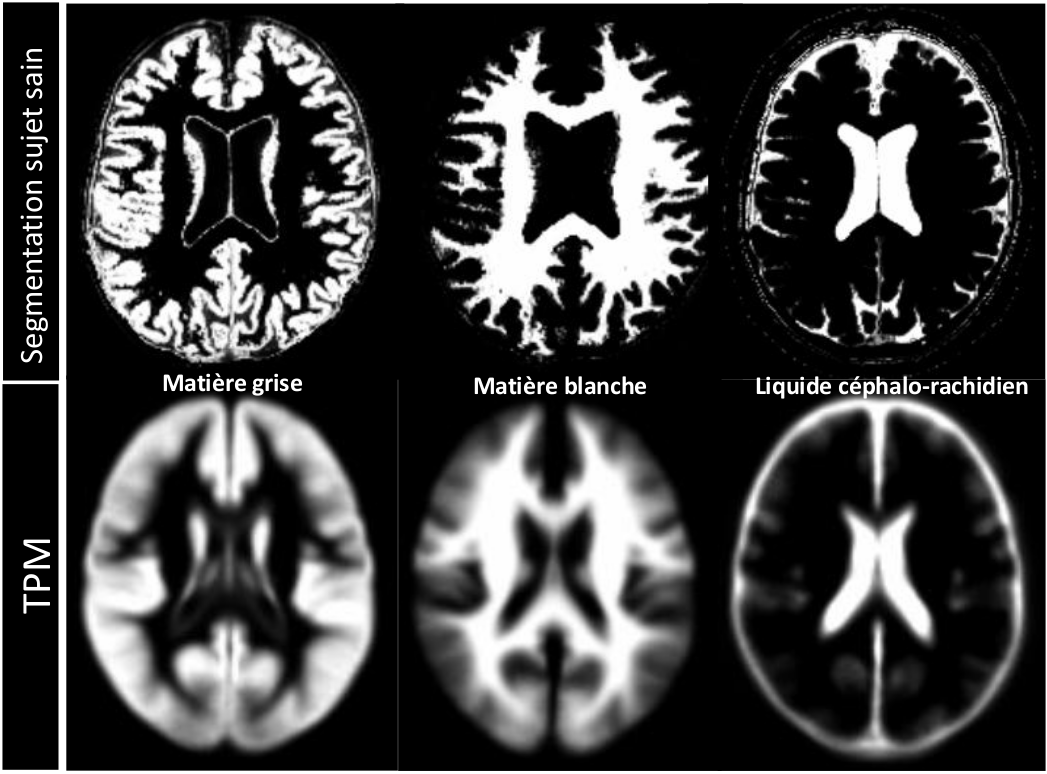
\includegraphics[width=10cm]{A_8_dartel}
\caption{Exemple de segmentation DARTEL sur un sujet sain, et TPM utilisées.}
\label{fig:A_8_dartel}	
\end{figure}
\section{Articles soumis ou acceptés}
\begin{itemize}
\item {\em Quantitative susceptibility mapping in superficial hemosiderosis of the central nervous system}.
Dargazanli C, {\bf Deverdun J}, Lionnet C, Michau S, Ozluk E, Corlobé A, Ayrignac X, Carra-Dallière
 C, Le Bars E, Labauge P, Bonafé A, Menjot de Champfleur N. J {\em Neuroradiol.} 06/2015 ;
\item {\em Quantitative susceptibility mapping suggests a paramagnetic effect in PML}. Clarisse Carra-
Dalliere, Nicolas Menjot de Champfleur, Xavier Ayrignac, {\bf Deverdun J}, Pierre Labauge.
{\em Neurology} 04/2015;
\item {\em SEP cavitaires et CACH : apport de l’IRM dans le diagnostic différentiel.} Xavier Ayrignac, Nicolas
  Menjot De Champfleur, Sophie Menjot De Champfleur, Clarisse Carra-Dallière, {\bf Deverdun J}, Astrid Corlobe, Pierre Labauge. {\em Revue Neurologique} 04/2015 ;
\item {\em Diffusion Tensor Imaging Differentiates Vascular Parkinsonism From Parkinsonian Syndromes
of Degenerative Origin in Elderly Subjects}. {\bf Deverdun J}, Sophie Menjot de Champfleur,
 Simon Cabello-Aguilar, Florence Maury, François Molino, Mahmoud Charif, Nicolas Leboucq,
 Xavier Ayrignac, Pierre Labauge, Alain Bonafe, Giovanni Castelnovo, Emmanuelle Le Bars,
Christian Geny, Nicolas Menjot de Champfleur. {\em European Journal of Radiology} 11/2014;
\item {\em Functional reorganization of the attentional networks in low-grade glioma patients: A
   longitudinal study.} Pom Charras, Guillaume Herbet, {\bf Deverdun J}, Nicolas Menjot de
    Champfleur, Hugues Duffau, Paolo Bartolomeo, François Bonnetblanc. {\em Cortex} 08/2014;
\item {\em Role of fronto-striatal tract and frontal aslant tract in movement and speech: an axonal
   mapping study.} Masashi Kinoshita, Nicolas Menjot de Champfleur, {\bf Deverdun J}, Sylvie
  Moritz-Gasser, Guillaume Herbet, Hugues Duffau. {\em Brain Structure and Function} 08/2014;
\item {\em Working Memory activation of neural networks in the elderly as a function of information
   processing phase and task complexity.} Céline Charroud, Jason Steffener, Emmanuelle Le Bars,
   {\bf Deverdun J}, Alain Bonafe, Meriem Abdennour, Florence Portet, François Molino, Yaakov
     Stern, Karen Ritchie, Nicolas Menjot de Champfleur, Tasnime N. Akbaraly. {\em Soumis à Journal of
     Cognitive Neuroscience};
\item {\em Corpus callosum integrity in mood disorders is associated with the history of suicide attempts.}
   Cyprien, Fabienne; Menjot de Champfleur, Nicolas; {\bf Deverdun J}; Olié, Emilie; Le Bars,
   Emmanuelle; Bonafé, Alain; Mura, Thibault; Jollant, Fabrice; Courtet, Philippe; Artero,
   Sylvaine. {\em Soumis à Bipolar disorders} ;
\item {\em Recovery of functional connectivity of the sensorimotor network after surgery for diffuse low-
   grade gliomas involving supplementary motor area.} Matthieu Vassal, Céline Charroud, {\bf Deverdun J}, Emmanuelle Le Bars, François Molino, François Bonnetblanc, Anthony Boyer,
      Anirban Dutta, Guillaume Herbet, Sylvie Moritz-Gasser, Alain Bonafé, Hugues Duffau, Nicolas
      Menjot de Champfleur, {\em Soumis à Brain Topography};
\item {\em Use of Quantitative Susceptibility Mapping (QSM) in Progressive Multifocal
   Leukoencephalopathy.} C. Carra-Dalliere, N. Menjot de Champfleur, {\bf Deverdun J}, X. Ayrignac,
  E. Nerrant, A. Makinson, M.L. Casanova, P. Labauge. {\em Soumis à JNNP} ;
\item {\em Large-Scale Reorganization Of The Language Network Functional Connectivity Induced By Low-
   Grade Glioma Resection.} Nicolas Menjot de Champfleur; Guillaume Herbet; Sylvie Moritz-
  Gasser; Igor Lima Maldonado; {\bf Deverdun J}; François Molino; Emmanuelle Le Bars; Alain
    Bonafé; Hugues Duffau. {\em Soumis à European Radiology}
\item {\em Subcortical longitudinal changes in spontaneous neuronal activity after wide-awake surgery of
   brain tumours: a resting state fMRI study.} Anthony Boyer, {\bf Deverdun J}, Hugues Duffau,
    Emmanuelle Le Bars, Nicolas Menjot de Champfleur, François Bonnetblanc. {\em Soumis à HBM} ;
\item {\em The experience of social exclusion in women with a history of suicidal acts: a neuroimaging
study.} E. Olié, N. Menjot de Champfleur, F. Cyprien, E. Le Bars, {\bf Deverdun J}, T. Mura, A. Bonafé,
 F. Jollant, P. Courtet ; {\em Soumis}
\item {\em MR volumetric morphometry is a diagnostic tool of vascular parkinsonism in elderly subjects.}
   Vincent Dunet$\ast$, {\bf Deverdun J}$\ast$, Celine Charroud, Emmanuelle Le Bars, Francois Molino,
  Sophie Menjot de Champfleur, Florence Maury, Mahmoud Charif, Xavier Ayrignac, Pierre
 Labauge, Giovanni Castelnovo, Frederic Pinna, Alain Bonafe, Nicolas Leboucq, Christian Geny,
Nicolas Menjot de Champfleur. {\em Soumis à Brain};
\item {\em Quantitative susceptibility mapping in patients with parkinsonism: comparison to diffusion
   tensor imaging.} V. Dunet, {\bf Deverdun J}, C. Charroud, C. Geny, F. Molino, S. Menjot de
  Champfleur, F. Maury, M. Charif, P. Labauge, X. Ayrignac, G. Castelnovo, F. Pinna, A. Bonafé,
  N. Leboucq, E. Le Bars, and N. Menjot de Champfleur. {\em Soumis dans Brain}.
\item {\em Mean arterial pressure change associated with cerebral blood flow in healthy elderly subjects.}
   {\bf Deverdun J}, Tasnime N. Akbaraly, Celine Charroud, Meriem Abdennour, Adam M.
  Brickman, Stephane Chemouny, Jason Steffener, Florence Portet, Alain Bonafe, Yaakov Stern,
 Karen Ritchie, François Molino, Emmanuelle Le Bars, Nicolas Menjot de Champfleur. {\em Soumis à
  JCFBM};
\item {\em Role of the left frontal aslant tract in stuttering: A brain stimulation and tractographic study.}
   Rahsan Kemerdere, Nicolas Menjot de Champfleur, Guillaume Herbet,{\bf Deverdun J},
    Jérôme Cochereau, Sylvie Moritz-Gasser et Hugues Duffau. {\em Préparation pour soumission.}
\end{itemize}
















\bibliography{jeremythesebib}{}
\bibliographystyle{francaissc}